\documentclass{article}

\usepackage{microtype}
\usepackage{graphicx}
\usepackage{subcaption}
\usepackage{xcolor}
\usepackage{booktabs}
\usepackage{multirow}
\usepackage{listings}
\usepackage{tikz}
\usetikzlibrary{arrows.meta,positioning,calc,fit,backgrounds,patterns}
\usepackage[hyphens]{url}
\usepackage[breaklinks=true]{hyperref}
\Urlmuskip=0mu plus 3mu

% Use accepted style (no review footer)
\usepackage[accepted]{icml2026}
\makeatletter
\renewcommand{\Notice@String}{}
\makeatother

\widowpenalty=10000
\clubpenalty=10000
\brokenpenalty=10000
\hyphenpenalty=5000
\exhyphenpenalty=5000
\tolerance=3000
\emergencystretch=3em
\setlength{\parfillskip}{0pt plus 0.75\textwidth}

\icmltitlerunning{Intrinsic Preferences of AI Coding Agents Under Underspecified Prompts}

\begin{document}

\twocolumn[
  \icmltitle{Intrinsic Preferences of AI Coding Agents:\\Thematic Priors, Fixation, and Defaults Under Underspecified Prompts}

  \begin{icmlauthorlist}
    \icmlauthor{Changkun Ou}{lmu,latere}
  \end{icmlauthorlist}

  \icmlaffiliation{lmu}{LMU Munich, Germany}
  \icmlaffiliation{latere}{Latere AI, \url{https://latere.ai}}

  \icmlcorrespondingauthor{Changkun Ou}{research@changkun.de}

  \icmlkeywords{AI coding agents, autonomous behavior, LLM evaluation, model priors, prompt sensitivity, thematic fixation}

  \vskip 0.3in
]

\printAffiliationsAndNotice{}

\begin{abstract}
What do AI coding agents build when given no specification?
Motivated by a production deployment where an autonomous pipeline
plateaued into micro-optimizations, we conducted a controlled
study across 725~sessions spanning 34~models from 8~labs,
2~agent harnesses, 5~prompts, and multiple harness versions.
We document four phenomena. (1)~\textbf{Factor sensitivity is
large}: prompt wording determines whether agents propose or
implement, whether outputs are 30 or 600~LOC, and whether targets
are terminal or browser. (2)~\textbf{Models have behavioral
attractors}: under a volitional prompt (``Just do something you
want''), models return to a characteristic artifact, with Conway's
Game of Life recurring across models from three different labs,
and the attractor shifting with model generation rather than
staying fixed. (3)~\textbf{Holding the model and varying the
harness separates model traits from scaffold artifacts}: output
medium and topic are largely properties of the model, surviving a
change of agent scaffold, with one clean counterexample
(\texttt{kimi-k3}, terminal 4/5 under one harness and browser 4/5
under the other). (4)~\textbf{Small cells overstate fixation}:
re-running one model at 50~sessions per cell puts its attractor
near 22\% of runs rather than the 80--100\% that 5-run cells
suggest, and dissolves a cross-harness contrast that the 5-run
version of the same comparison had reported. The mechanism
survives this correction, since 22\% mass on one specific program
out of an unbounded space is still a highly peaked distribution,
but the magnitude does not. These findings suggest conventional
benchmarks may not capture decision-making behavior in
underspecified regimes where agents are increasingly deployed. We
release all experimental infrastructure and data.
\end{abstract}

%% ============================================================
\section{Introduction}
\label{sec:intro}

Autonomous AI coding agents such as
Devin~\citep{cognition2024devin} and coding assistants like Claude
Code~\citep{anthropic2025claudecode}, OpenAI Codex
CLI~\citep{openai2025codex}, and
Cursor~\citep{cursor2024}, now resolve over 80\% of real-world
GitHub issues on SWE-bench
Verified~\citep{swebenchpro2026,jimenez2024swebench,yang2024sweagent},
with the Stanford AI Index reporting agent task success jumping
from 12\% to 66\% in a single year~\citep{stanforhai2026index}.
These results come from \emph{well-specified} tasks: fix this
bug, implement this feature, pass this test suite. Increasingly,
however, agents are deployed in regimes where the task is
under-specified: long-running autonomous loops, vague user
requests, ambient agents acting in the background. What an agent
\emph{chooses} to do in such regimes is not directly measured by
current benchmarks.

Our motivation is practical. We deployed a four-stage autonomous
pipeline (strategist, executor, tester, documenter) on a
production codebase for 10 days. Output was initially
impressive, 627 commits, growing from 25K to 122K LOC, then
plateaued into a \emph{micro-optimization spiral} of locally
optimal, globally irrelevant
refinements~\citep{christensen1997,simon1956}. Ablating the
pipeline to a single agent revealed model-level defaults
(Claude $\to$ Game of Life, GPT $\to$ todo apps) that were
reproducible but tangled with prompt wording and environment
context. We could not tell, from the deployment alone, how much
of what we saw was a property of the model versus an artifact of
the setup. So we ran a controlled sweep.

This paper is an empirical study of what AI coding agents
produce under underspecified prompts. Across 725~sessions
spanning 34~models from 8~labs, 2~agent harnesses, 5~prompts, and
multiple harness versions, we report four observations:

\textbf{(1)~Factor sensitivity is large.} Prompt wording
determines whether models propose or implement; whether outputs
are 30 or 600~LOC; whether targets are terminal or browser;
whether runs fixate or diversify. Environment artifacts shift
language selection from polyglot to Python-dominant. Harness
version modulates fixation strength and complexity
independently of the model.

\textbf{(2)~A volitional prompt concentrates the signal.} A
one-sentence directive (``Just do something you want.''),
stripped of project reference and goal framing, produced the
sharpest preference signal in the study: opus-4.6 chose
Conway's Game of Life in 5 of 5 runs; opus-4.7 chose the
Mandelbrot set in 5 of 5 runs; implementations converged to
near-identical LOC and structure within each model.

\textbf{(3)~Varying the harness separates model traits from
scaffold artifacts.} Holding the model fixed and swapping the
agent scaffold (Experiments~12--19) leaves both the output medium
and the topic family largely intact: Claude models stay in the
terminal and GPT models stay in the browser under \emph{both}
harnesses. One model breaks this, and it breaks it cleanly:
\texttt{kimi-k3} builds terminal programs in 4 of 5 runs under one
harness and browser pages in 4 of 5 under the other, with the
container image held fixed. Medium is therefore usually, but not
necessarily, a property of the model.

\textbf{(4)~Five-run cells overstate fixation, and cannot support
cross-cell comparison.} Experiment~20 re-runs a single model at
50~sessions per cell across three cells (150~sessions). Its
attractor appears in ${\sim}22\%$ of runs, not the 80--100\%
that 5-run cells report; and a cross-harness difference that the
5-run version of the same comparison had presented as a finding
disappears entirely, with no pair of cells differing significantly.
We treat this as a calibration result for the rest of the study:
single-cell frequencies are informative, differences between two
5-run cells are not.

\textbf{Sibling models split cleanly on theme.} Both Opus
preferences are classical-CS touchstones that express complex
behavior from simple rules, but they fall on different sides of
a legible axis: opus-4.6 toward \emph{self-reference}
(cellular automata, ray tracing, typing tests), opus-4.7 toward
\emph{emergence} (flocking, reaction-diffusion, maze and
dungeon generation). A replication on a newer harness
(Experiment~8, adding opus-4.8) shows the \emph{robustness} of
this fixation is model-specific: opus-4.6 reproduces Game of
Life 5/5 while opus-4.7 disperses across the family and the new
opus-4.8 only loosely clusters. What survives is the thematic
family, not the single artifact.

We report these as empirical observations, not as a theory of
model priors or a proposed benchmark. Most cells use $n=5$, and
Experiment~20 quantifies what that costs: such cells establish
that an attractor \emph{exists} but cannot compare two conditions.
Where this paper reasons from a difference between two 5-run
cells, we mark the direction as provisional. The robustness checks
still outstanding (paraphrase stability, temperature variation,
functional verification) are enumerated in
\S\ref{sec:limitations}.

%% ============================================================
\section{Related Work}
\label{sec:related}

\paragraph{Code generation benchmarks.}
HumanEval~\citep{chen2021codex} and MBPP~\citep{austin2021mbpp}
evaluate function-level code generation from docstrings.
SWE-bench~\citep{jimenez2024swebench} scales to repository-level
bug fixes. More recent benchmarks push further:
ABC-Bench~\citep{zhang2026abcbench} requires agents to manage the
full backend development lifecycle across 8~languages and
19~frameworks, and NL2Repo-Bench~\citep{nl2repobench2025} evaluates
long-horizon repository generation from natural language
descriptions. SWE-bench Pro~\citep{swebenchpro2026} addresses
contamination concerns with 1,865 multi-language tasks where
models scoring 80\%+ on Verified only reach 46--57\%.
All these benchmarks share one property: a well-specified task
with a ground-truth solution. Our work complements them by
removing the specification entirely, measuring what agents do when
the ``what to build'' decision is theirs.

\paragraph{Autonomous agent loops.}
AutoGPT~\citep{significantgravitas2023autogpt} and
BabyAGI~\citep{nakajima2023babyagi} pioneered open-ended
autonomous agent loops, where an LLM iteratively proposes and
executes tasks toward a high-level objective. In practice, these
systems frequently enter infinite loops, spiral into costly API
calls, and struggle to determine termination conditions.
More recent frameworks like SAGA~\citep{saga2025goalevolving}
employ bi-level architectures where outer-loop agents evolve
objectives while inner loops optimize under them, and
CORAL~\citep{coral2026multiagent} replaces rigid control with
persistent memory and asynchronous multi-agent collaboration.
Our production deployment exhibits many of the same failure modes
reported in these systems, but we go further by systematically
isolating the factors that drive them.

\paragraph{Agent reliability and behavioral collapse.}
Recent work on long-horizon agents has documented
\emph{meltdown behavior}, where agents transition from coherent
to incoherent looping over extended task
horizons~\citep{beyondpass2026}. Aggregate pass@1 drops from
76.3\% at short horizon to 52.1\% at very long horizon, a
24-point decline. Our micro-optimization spiral is a related
phenomenon at a longer timescale: the agent does not become
incoherent, but its decisions become increasingly locally optimal
and globally irrelevant.

\paragraph{Prompt sensitivity.}
LLM outputs are sensitive to prompt
phrasing~\citep{lu2022promptorder,zhao2021calibrate}. Our work
extends this to autonomous agents, where prompt changes affect
not just output text but \emph{behavioral patterns}: whether the
agent proposes or implements, what topic it selects, and how
complex its output is.

\paragraph{Model behavioral tendencies.}
Studies of LLM biases~\citep{santurkar2023opinions} have shown that
models exhibit consistent preferences. Recent work demonstrates
that LLMs display human-like social desirability biases in
personality assessments~\citep{simonds2025llmpersonality} and
develop emergent social conventions in multi-agent
populations~\citep{chuang2024emergent}. These findings suggest that
``personality-like'' profiles in LLMs are reproducible yet
context-dependent. We document an analogous phenomenon in coding
agents: persistent topical fixations that survive across prompt
variations and repeated runs, and that differ across model
versions in ways consistent with stable thematic priors.

\paragraph{Text degeneration and repetition.}
Neural text generation is prone to degenerate repetition, where
models enter loops producing the same tokens or
phrases~\citep{holtzman2020curious}. The fixation we observe
operates at a higher level of abstraction: the agent does not
repeat tokens but repeatedly \emph{chooses the same project}.
This is closer to mode collapse in generative models than to
token-level degeneration, suggesting that the decision of what to
build has a narrower effective distribution than the space of
possible implementations.

\paragraph{Bounded rationality and satisficing.}
Simon's theory of bounded rationality~\citep{simon1956} argues that
agents with limited computational resources settle for satisfactory
rather than optimal solutions. Christensen's innovator's
dilemma~\citep{christensen1997} describes how incumbents
over-optimize along existing trajectories. We observe both
patterns: without external disruption, agent systems satisfice
within their initial framing, producing incremental improvements
that crowd out structurally novel alternatives.

%% ============================================================
\section{Experiment Setup}
\label{sec:setup}

Our investigation proceeds in two stages: a production deployment
with ablation studies (\S\ref{sec:trail}), and controlled
single-session experiments (\S\ref{sec:controlled}).

\subsection{Production Deployment and Ablation}
\label{sec:trail}

We summarize the production deployment that motivated the
study; full details and logs are in the open-source
repository. A four-stage agent pipeline (Strategist,
Executor, Tester, Documenter, looping autonomously)
operated on a production codebase for 10 days
(March~7--16, 2026), producing 627~commits and growing the
codebase from 25K to 122K~LOC, before plateauing into the
\emph{micro-optimization spiral} described in \S\ref{sec:intro}.

Systematic ablation (Figure~\ref{fig:ablation}) isolated
which pipeline components mattered and, relevant for
what follows, revealed model-specific defaults under the
single-agent configuration: Claude (Opus~4.6) consistently
chose Game of Life; GPT models defaulted to todo list
applications. Without the Documenter, the Strategist lost
historical context and reproposed completed work. Without
the Tester, the system grew a single Game of Life
implementation to 112K~LOC in one file, then broke
12K~lines in a refactor with no mechanism to detect the
regression. Single-agent defaults were stable across
repetitions but tangled with environment context and prompt
wording, motivating the controlled experiments in
\S\ref{sec:controlled}.

\begin{figure}[t]
\centering
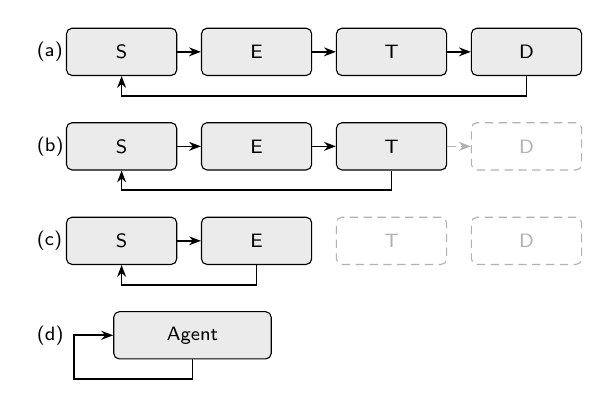
\begin{tikzpicture}[
  node distance=4mm and 3mm,
  stage/.style={draw, rounded corners=2pt, minimum width=14mm,
    minimum height=6mm, font=\scriptsize\sffamily, fill=black!8},
  removed/.style={stage, fill=white, draw=black!30,
    text=black!30, densely dashed},
  arr/.style={-{Stealth[length=1.5mm]}, semithick},
  arrd/.style={-{Stealth[length=1.5mm]}, semithick, black!30,
    densely dashed},
  lbl/.style={font=\scriptsize\sffamily, anchor=west},
]
% (a) Full pipeline
\node[lbl] at (-1.2,0) {(a)};
\node[stage] (S1) at (0,0) {S};
\node[stage, right=of S1] (E1) {E};
\node[stage, right=of E1] (T1) {T};
\node[stage, right=of T1] (D1) {D};
\draw[arr] (S1)--(E1); \draw[arr] (E1)--(T1);
\draw[arr] (T1)--(D1);
\draw[arr] (D1.south)--++(0,-2.5mm)-|([xshift=0mm]S1.south);

% (b) No Documenter
\node[lbl] at (-1.2,-1.2) {(b)};
\node[stage] (S2) at (0,-1.2) {S};
\node[stage, right=of S2] (E2) {E};
\node[stage, right=of E2] (T2) {T};
\node[removed, right=of T2] (D2) {D};
\draw[arr] (S2)--(E2); \draw[arr] (E2)--(T2);
\draw[arrd] (T2)--(D2);
\draw[arr] (T2.south)--++(0,-2.5mm)-|([xshift=0mm]S2.south);

% (c) No Tester
\node[lbl] at (-1.2,-2.4) {(c)};
\node[stage] (S3) at (0,-2.4) {S};
\node[stage, right=of S3] (E3) {E};
\node[removed, right=of E3] (T3) {T};
\node[removed, right=of T3] (D3) {D};
\draw[arr] (S3)--(E3);
\draw[arr] (E3.south)--++(0,-2.5mm)-|([xshift=0mm]S3.south);

% (d) Single agent
\node[lbl] at (-1.2,-3.6) {(d)};
\node[stage, minimum width=20mm] (A) at (0.9,-3.6) {Agent};
\draw[arr] (A.south) -- ++(0,-2.5mm) -|
  ([xshift=-5mm]A.west) -- (A.west);
\end{tikzpicture}
\caption{Ablation configurations. S\,=\,Strategist,
  E\,=\,Executor, T\,=\,Tester, D\,=\,Documenter.
  (a)~Full pipeline. (b)~Without Documenter: lost memory.
  (c)~Without Tester: unchecked regressions.
  (d)~Single agent: reveals model priors.}
\label{fig:ablation}
\end{figure}

\subsection{Controlled Single-Session Experiments}
\label{sec:controlled}

We test 34 models from 8 labs (Table~\ref{tab:models}), accessed
through a unified API gateway. Two containerized agent harnesses
provide execution environments: the \textbf{Claude Code harness}
runs Anthropic's CLI with a full Linux environment; the
\textbf{codex harness} runs OpenAI's Codex CLI under bubblewrap
isolation. From Experiment~16 onward both run from a single shared
image, so the harness can be swapped with every other component of
the container held byte-identical.

Models outside a harness's native provider reach it through the
gateway's \emph{compatibility surfaces}, which translate dialects:
\texttt{/compat/anthropic} presents an arbitrary model through the
Anthropic Messages API (letting the Claude Code harness drive
non-Anthropic models), and \texttt{/compat/openai} presents one
through the OpenAI Responses API (letting the codex harness drive
non-OpenAI models). Building these two surfaces is what makes the
harness a manipulable variable rather than a fixed confound of the
provider, and Experiments~12--20 depend on them.

Each session starts with a fresh, empty workspace and a fresh
agent configuration directory. Environment bias is controlled by
disabling pre-installed tools (specifically RTK~\citep{rtk2025})
via a no-op stub, and prompt caching is disabled on the Claude
Code side.

\begin{table}[t]
\caption{The 34 models tested, by lab. Experiment numbers mark
  where a model first appears; models without a note were used in
  the early prompt sweeps (Exp1--3).}
\label{tab:models}
\small\resizebox{\columnwidth}{!}{%
\begin{tabular}{llp{3.6cm}}
\toprule
Lab & Model ID & Notes \\
\midrule
\multirow{10}{*}{Anthropic}
  & claude-opus-5     & Frontier (Exp18) \\
  & claude-fable-5    & Image-emitting habit (Exp8) \\
  & claude-sonnet-5   & Newest Sonnet (Exp9, 15) \\
  & claude-opus-4.8   & (Exp8) \\
  & claude-opus-4.7   & (Exp4--8) \\
  & claude-opus-4.6   & Primary comparison point \\
  & claude-opus-4.5   & Previous generation \\
  & claude-sonnet-4.6 & Mid-tier, prev gen (Exp9) \\
  & claude-sonnet-4.5 & Mid-tier, previous gen \\
  & claude-haiku-4.5  & Smallest Claude model \\
\midrule
\multirow{4}{*}{Google}
  & gemini-3-pro      & Latest Gemini Pro \\
  & gemini-3-flash    & Latest Gemini Flash \\
  & gemini-2.5-pro    & Previous generation \\
  & gemini-2.0-flash  & Older generation \\
\midrule
\multirow{12}{*}{OpenAI}
  & gpt-5.6-sol       & Reasoning (Exp11, 14) \\
  & gpt-5.6-terra     & Reasoning (Exp11, 14) \\
  & gpt-5.6-luna      & Reasoning (Exp11, 14) \\
  & gpt-5.5-pro       & Reasoning (Exp10) \\
  & gpt-5.5           & Large (Exp10) \\
  & gpt-5.4           & Later, largest \\
  & gpt-5.1           & Later, mid-tier \\
  & gpt-5-mini        & Later, small \\
  & gpt-5-nano        & Later, smallest \\
  & gpt-4o            & Previous generation \\
  & gpt-4.1           & Previous generation \\
  & gpt-4.1-mini      & Previous, small \\
\midrule
Zhipu    & glm-5.2, glm-5.1        & Open weights (Exp12/13) \\
Alibaba  & qwen3.7-max             & Open weights (Exp12/13) \\
MiniMax  & minimax-m3              & Open weights (Exp12/13) \\
DeepSeek & deepseek-v4-pro         & Open weights (Exp12/13) \\
         & deepseek-v4-flash-0731  & Scale cell (Exp19/20) \\
Moonshot & kimi-k2.7-code          & Open weights (Exp12/13) \\
         & kimi-k3                 & Medium counterexample (Exp16/17) \\
\bottomrule
\end{tabular}}
\end{table}

Five prompts progressively reduce task specification.
Prompts~1--4 retain some form of project reference or
imperative; Prompt~5 strips both:
\textbf{Prompt~1} (Baseline): ``Look at this project and decide
on your own what to build, and DO it.''
\textbf{Prompt~2} (Goal-focused): adds ``propose exactly ONE
goal'' and ``pick a concrete, interesting idea.''
\textbf{Prompt~3} (Implementation demand): adds ``JUST DO IT''
after Experiment~2 revealed that some models proposed without
implementing.
\textbf{Prompt~4} (Bare imperative): ``Build something. Just do
it.,'' the implementation demand with project reference
removed.
\textbf{Prompt~5} (Volitional): ``Just do something you
want.,'' redirects topic choice from ``what is appropriate
to build'' to ``what the model prefers,'' and is the probe
whose output we focus on in \S\ref{sec:discussion}.
Prompt~1 was used with RTK inadvertently present;
Prompts~2--5 ran with RTK disabled.

\paragraph{Execution matrix.}
The study runs in four phases. \textbf{Prompt phase (Exp1--7,
405~sessions):} Exp1, 14 models $\times$ 2 harnesses $\times$ 5
runs (140); Exp2, Claude Code only (70); Exp3, both harnesses
(140); Exp4, opus-4.7 on harness 2.1.109 (5); Exp5, opus-4.6 and
4.7 on 2.1.112 (10); Exp6, the same pair with Prompt~4 (10); Exp7,
the same pair with Prompt~5 (10) plus 20 supplementary Prompt~3
sessions for the other four Claude models.
\textbf{Model phase (Exp8--11, 55~sessions):} Exp8, opus-4.6/4.7/4.8
on harness 2.1.154 (15, later joined by 5 fable-5 sessions on a
bumped stack); Exp9, sonnet-4.6 and sonnet-5 on the Exp8 stack
(10); Exp10, gpt-5.5 and gpt-5.5-pro on codex (10); Exp11, three
gpt-5.6 variants on codex at matched \texttt{high} effort (15).
\textbf{Harness phase (Exp12--19, 115~sessions):} Exp12/13, the
same six open-weights models on each harness (30 + 30); Exp14,
the gpt-5.6 family on Claude Code (15); Exp15, opus-4.6 and
sonnet-5 on codex at matched effort (10); Exp16/17,
\texttt{kimi-k3} on each harness with the image held fixed (5 + 5);
Exp18, \texttt{claude-opus-5} on both harnesses (10); Exp19,
\texttt{deepseek-v4-flash-0731} on both harnesses (10).
\textbf{Scale phase (Exp20, 150~sessions):} the Exp19 model at 50
sessions per cell across three cells---Claude Code, codex at
\texttt{high} effort, and codex at \texttt{low}. Total: 725
sessions (Figure~\ref{fig:matrix}).

\begin{figure}[t]
\centering
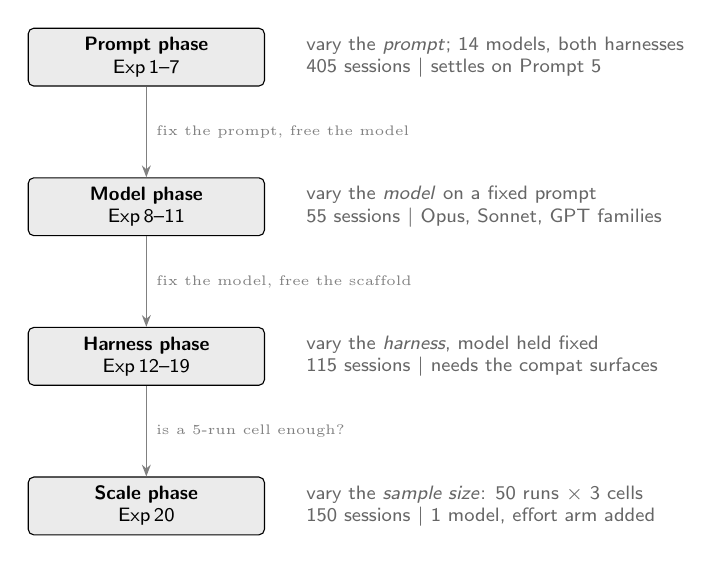
\begin{tikzpicture}[
  font=\scriptsize\sffamily,
  phase/.style={draw, rounded corners=2pt, minimum height=7mm,
    minimum width=30mm, fill=black!8, align=center},
  dim/.style={font=\scriptsize\sffamily, text=black!60, align=left},
  arr/.style={-{Stealth[length=1.5mm]}, semithick, black!50},
]
\node[phase] (P1) at (0,0)    {\textbf{Prompt phase}\\Exp\,1--7};
\node[phase] (P2) at (0,-1.9) {\textbf{Model phase}\\Exp\,8--11};
\node[phase] (P3) at (0,-3.8) {\textbf{Harness phase}\\Exp\,12--19};
\node[phase] (P4) at (0,-5.7) {\textbf{Scale phase}\\Exp\,20};

\node[dim, right=4mm of P1.east, anchor=west]
  {vary the \emph{prompt}; 14 models, both harnesses\\
   405 sessions \textbar{} settles on Prompt~5};
\node[dim, right=4mm of P2.east, anchor=west]
  {vary the \emph{model} on a fixed prompt\\
   55 sessions \textbar{} Opus, Sonnet, GPT families};
\node[dim, right=4mm of P3.east, anchor=west]
  {vary the \emph{harness}, model held fixed\\
   115 sessions \textbar{} needs the compat surfaces};
\node[dim, right=4mm of P4.east, anchor=west]
  {vary the \emph{sample size}: 50 runs $\times$ 3 cells\\
   150 sessions \textbar{} 1 model, effort arm added};

\draw[arr] (P1.south) -- node[right, font=\tiny, text=black!50]
  {fix the prompt, free the model} (P2.north);
\draw[arr] (P2.south) -- node[right, font=\tiny, text=black!50]
  {fix the model, free the scaffold} (P3.north);
\draw[arr] (P3.south) -- node[right, font=\tiny, text=black!50]
  {is a 5-run cell enough?} (P4.north);
\end{tikzpicture}
\caption{Experiment design, grouped by the factor each phase
  varies. Each phase was informed by the previous one: the prompt
  sweep identifies the volitional probe, the model sweep shows the
  probe yields per-model attractors, the harness sweep asks whether
  those attractors belong to the model or the scaffold, and the
  scale phase asks whether 5-run cells can support the comparisons
  the previous phase makes. Total: 725 sessions across 34 models.}
\label{fig:matrix}
\end{figure}

\paragraph{Metrics.}
For each session we record: topic (manually classified), tech
stack, complexity (files, LOC, function count), engineering
maturity (tests, README, build config, CI), and runtime (exit
code, wall-clock duration). Sessions with technical errors (exit
$\neq$ 0) are excluded from complexity metrics but included in
topic/fixation analysis when partial output reveals the model's
intent.

%% ============================================================
\section{Results}
\label{sec:results}

\subsection{Phase 1 --- Varying the Prompt (Exp1--7)}
\label{sec:phase-prompt}

The first phase holds the model set roughly constant and sweeps
the prompt from a project-referential instruction down to a bare
volitional one. Its purpose is to find a probe that elicits a
model's own choice rather than its reading of a task.

\subsubsection{Experiment~1: Baseline with Environment Bias}

Experiment~1 ran all 14 models on both backends with Prompt~1.
RTK was inadvertently present in the sandbox.
Eight models produced working code on the Claude backend
(Table~\ref{tab:exp1}). Claude models exhibited polyglot behavior
(Go, Rust, Python, JavaScript, TypeScript) and built developer
tools influenced by the RTK context. Gemini models produced
smaller output (61--89~LOC). All GPT models failed due to API
parameter incompatibility. On the Codex backend, all models
failed.

\begin{table}[t]
\caption{Experiment~1 (Claude backend). N\,=\,sessions without
  technical error. RTK present, biased toward dev tooling.}
\label{tab:exp1}
\small\resizebox{\columnwidth}{!}{%
\begin{tabular}{lrrlp{3cm}}
\toprule
Model & N & Avg LOC & Lang & Typical Project \\
\midrule
claude-sonnet-4.5  & 5 & 776 & Python & Dev workflow tools \\
claude-opus-4.6    & 5 & 607 & Go/Rust & TUI apps \\
claude-sonnet-4.6  & 5 & 506 & Python & Git/dev tools \\
claude-haiku-4.5   & 5 & 233 & Py/Go/TS & Developer utilities \\
claude-opus-4.5    & 5 & 221 & Go/JS/Py & CLI utilities \\
\midrule
gemini-3-flash     & 5 & 61 & JS/Go/Py & Small utilities \\
gemini-2.5-pro     & 5 & 64 & Python & Simple scripts \\
gemini-2.0-flash   & 3 & 89 & Python & Minimal scripts \\
\bottomrule
\end{tabular}}
\end{table}

\subsubsection{Experiment~2: Removing Environment Bias}

Disabling RTK and using Prompt~2 on the Claude backend caused a
dramatic shift (Table~\ref{tab:exp2}): from developer tools to
games, visualizations, and productivity apps. All Claude models
converged on Python. The ``propose ONE goal'' framing caused
claude-haiku-4.5 and opus-4.5 to propose ideas without generating
code (a \emph{planning trap}).

\begin{table}[t]
\caption{Experiment~2 (Claude backend, RTK disabled).}
\label{tab:exp2}
\small\resizebox{\columnwidth}{!}{%
\begin{tabular}{lrrlp{3cm}}
\toprule
Model & N & Avg LOC & Lang & Typical Project \\
\midrule
claude-sonnet-4.6  & 5 & 204 & Python & Diverse interactive tools \\
claude-sonnet-4.5  & 5 & 234 & Python & Games + task managers \\
claude-opus-4.6    & 4 & 408 & Python & Game of Life (every run) \\
gemini-3-flash     & 5 & 86  & Go/Py/JS & Small CLI tools \\
gemini-2.5-pro     & 4 & 57  & Python & Simple utilities \\
gemini-2.0-flash   & 3 & 16  & Python & Hello World \\
claude-opus-4.5    & 5 & 291 & Python & Habit trackers (2 impl., 3 proposed) \\
claude-haiku-4.5   & 5 & 160 & Node.js & 1 impl., 4 proposed only \\
\bottomrule
\end{tabular}}
\end{table}

\subsubsection{Experiment~3: Breaking the Planning Trap}

Adding ``JUST DO IT'' to the prompt and running both backends
(Tables~\ref{tab:exp3_claude}--\ref{tab:exp3_codex}) transformed
haiku from proposing without implementing to the
highest-maturity model: READMEs in every run, tests in 40\%,
average 6.4~files and 467~LOC.

\begin{table}[t]
\caption{Experiment~3: Claude backend, Anthropic models.}
\label{tab:exp3_claude}
\small\resizebox{\columnwidth}{!}{%
\begin{tabular}{lrrrrr}
\toprule
Model & N & Avg LOC & Files & Test\% & README\% \\
\midrule
haiku-4.5   & 5 & 467 & 6.4 & 40\% & 100\% \\
sonnet-4.6  & 5 & 307 & 1.2 & 0\%  & 0\%   \\
sonnet-4.5  & 3 & 380 & 3.5 & 0\%  & 75\%  \\
opus-4.5    & 3 & 467 & 3.0 & 0\%  & 67\%  \\
opus-4.6    & 4 & 322 & 1.0 & 0\%  & 0\%   \\
\bottomrule
\end{tabular}}
\end{table}

\begin{table}[t]
\caption{Experiment~3: Claude backend, GPT models via litellm.}
\label{tab:exp3_gpt_claude}
\small\resizebox{\columnwidth}{!}{%
\begin{tabular}{lrrrrr}
\toprule
Model & N & Avg LOC & Test\% & README\% & CI\% \\
\midrule
gpt-5-mini    & 5 & 121 & 100\% & 80\% & 80\% \\
gpt-4.1-mini  & 4 & 8   & 20\%  & 60\% & 0\%  \\
gpt-4.1       & 2 & 31  & 0\%   & 0\%  & 0\%  \\
gpt-5.4       & 1 & 7   & 0\%   & 100\% & 0\% \\
gpt-5.1       & 0 & n/a & n/a   & n/a  & n/a  \\
\bottomrule
\end{tabular}}
\end{table}

\begin{table}[t]
\caption{Experiment~3: Codex backend, GPT models (files not
persisted to host due to bwrap isolation).}
\label{tab:exp3_codex}
\small\resizebox{\columnwidth}{!}{%
\begin{tabular}{lrrlr}
\toprule
Model & N & Avg LOC & Typical Project & Test\% \\
\midrule
gpt-5.4       & 5 & 230 & Diverse (web apps, CLI) & 40\% \\
gpt-5.1       & 5 & 98  & CLI with packaging      & 40\% \\
gpt-4.1       & 5 & 56  & Todo list apps          & 40\% \\
gpt-5-mini    & 4 & 40  & Greeting utilities      & 60\% \\
gpt-4.1-mini  & 4 & 8   & Hello World             & 40\% \\
\bottomrule
\end{tabular}}
\end{table}

\paragraph{Model fixation.}
claude-opus-4.6 chose Conway's Game of Life in all 10 runs
across Exp2--3 (including error runs with partial files).
claude-sonnet-4.5 developed a Pomodoro fixation (3 of 4 completed
runs in Exp3). gpt-4.1 on Codex built todo apps in 3 of 5 runs.
In contrast, claude-sonnet-4.6 produced a different project in
every run across all three experiments, including creative uses
of the Claude API (commit generator, AI debate arena).

\paragraph{Backend inversion.}
GPT rankings inverted between backends. On Codex (native):
gpt-5.4~(230~LOC) $\gg$ gpt-5.1~(98) $>$ gpt-4.1~(56).
On Claude (via litellm): gpt-5-mini was the only productive model
(121~LOC with tests and CI), while gpt-5.4 and gpt-5.1
produced almost nothing. Wall-clock runtimes confirm the
difference: gpt-5-mini ran 193--1378s per session (indicating
iterative tool use), while other GPT models completed in 9--55s
(indicating minimal interaction).

\paragraph{Gemini models.}
Across all experiments, Gemini models were near-non-functional on
both backends. Only 1 of 20~runs on the Claude backend in Exp3
produced files.

\subsubsection{Experiment~4: Model Version Effect}

Experiment~4 tested claude-opus-4.7 with the same prompt and
harness as Exp3, isolating the model version
(Table~\ref{tab:exp4}).

\begin{table}[t]
\caption{Experiment~4: opus-4.7 (harness 2.1.109).}
\label{tab:exp4}
\small\resizebox{\columnwidth}{!}{%
\begin{tabular}{rlrr}
\toprule
Run & Topic & LOC & Dur. \\
\midrule
01 & Reaction-diffusion (Gray-Scott) & 570 & 369s \\
02 & Boids flocking & 367 & 135s \\
03 & Conway's Game of Life & 434 & 151s \\
04 & Maze generator + A* solver & 762 & 324s \\
05 & Dungeon generator (BSP) & 557 & 229s \\
\midrule
   & \textbf{Average} & \textbf{538} & \textbf{242s} \\
\bottomrule
\end{tabular}}
\end{table}

Opus~4.7 chose Game of Life only once, compared to opus-4.6's
10/10 fixation. All 5~runs produced distinct projects, all in the
simulation/visualization category. Average complexity nearly
doubled (538 vs.\ 322~LOC), and 2 of 5~runs included tests.

\subsubsection{Experiment~5: Harness Version Effect}

Experiment~5 re-ran both models on an upgraded harness (Claude
Code 2.1.112 vs.\ 2.1.109), isolating the harness as the
variable (Table~\ref{tab:exp5}).

\begin{table}[t]
\caption{Experiment~5: harness 2.1.112 (same prompt as Exp3--4).}
\label{tab:exp5}
\small\resizebox{\columnwidth}{!}{%
\begin{tabular}{llrrl}
\toprule
Model & Run & LOC & Dur. & Topic \\
\midrule
\multirow{5}{*}{opus-4.6}
  & 01 & 277 & 150s & Game of Life \\
  & 02 & 345 & 227s & Ray tracer (Blinn-Phong) \\
  & 03 & 341 & 138s & Game of Life \\
  & 04 & 626 & 214s & Typing speed test \\
  & 05 & 345 & 170s & Game of Life (Go) \\
\midrule
\multirow{5}{*}{opus-4.7}
  & 01 & 246 & 133s & Boids flocking \\
  & 02 & 315 & 77s  & Procedural dungeon (BSP) \\
  & 03 & 178 & 50s  & Maze generator + A* \\
  & 04 & 264 & 97s  & Boids flocking \\
  & 05 & 309 & 81s  & Boids flocking \\
\bottomrule
\end{tabular}}
\end{table}

Opus-4.6's Game of Life fixation dropped from 10/10 (harness
2.1.109) to 3/5 (2.1.112). Opus-4.7 gained a boids fixation
(3/5) that was absent on 2.1.109. Opus-4.7 averaged 262~LOC
(down from 538 in Exp4) with no tests, while opus-4.6 averaged
387~LOC (up from 322).

\subsubsection{Experiment~6: Prompt Reduction}

Experiment~6 replaced Prompt~3 with Prompt~4 (``Build something.
Just do it.''), removing the ``look at this project,'' the
prohibition on asking, and the goal framing, while holding models
and harness fixed (opus-4.6, opus-4.7, CC~2.1.112). The terse
imperative produced two unexpected shifts (Table~\ref{tab:exp6}):
output roughly halved in size, and 3 of 10~runs produced
HTML/Canvas pages rendered in a browser, an interactive particle
sandbox, a Perlin-noise flowfield, and a browser-based boids
simulation. This is the first non-terminal output observed across
Exp1--Exp5 ($\sim$275 sessions). The terminal-default we had
treated as invariant is therefore prompt-dependent: the
project-referential framing in earlier prompts appears to have
steered models toward terminal scripts; the bare imperative
widens the target to anything a single file can host.

\begin{table}[t]
\caption{Experiment~6: Prompt~4 (``Build something. Just do it.''),
  harness 2.1.112.}
\label{tab:exp6}
\small\resizebox{\columnwidth}{!}{%
\begin{tabular}{llrrl}
\toprule
Model & Run & LOC & Dur. & Topic \\
\midrule
\multirow{5}{*}{opus-4.6}
  & 01 & 206 & 44s & Particle sandbox (HTML/Canvas) \\
  & 02 & 138 & 39s & Game of Life (named patterns) \\
  & 03 & 68  & 27s & Game of Life \\
  & 04 & 216 & 46s & Fireworks (curses) \\
  & 05 & 72  & 28s & Game of Life \\
\midrule
\multirow{5}{*}{opus-4.7}
  & 01 & 119 & 42s & Game of Life \\
  & 02 & 211 & 61s & Flowfield (HTML/Canvas) \\
  & 03 & 231 & 56s & Boids (HTML/Canvas) \\
  & 04 & 122 & 48s & Game of Life (named patterns) \\
  & 05 & 116 & 43s & Game of Life \\
\bottomrule
\end{tabular}}
\end{table}

Opus-4.6 avg~LOC fell from 387 (Exp5) to 140 (Exp6); opus-4.7
from 262 to 160. Opus-4.7's fixation flipped from boids (Exp5,
3/5) to Game of Life (Exp6, 3/5) despite identical harness and
environment, further confirming that fixation target is
prompt-sensitive even within a single model and harness.

\subsubsection{Experiment~7: Preference Elicitation}

Experiment~7 used Prompt~5 (``Just do something you want.''),
which redirects from ``what is appropriate to build'' to ``what
the model prefers.'' The same two models (opus-4.6, opus-4.7) on
the same harness produced the strongest fixation signal in the
entire study (Table~\ref{tab:exp7}): opus-4.6 chose Conway's Game
of Life in 5 of 5 runs; opus-4.7 chose the Mandelbrot set in 5
of 5 runs. Both are classical CS touchstones that express complex
behavior from simple rules, yet the two models lock onto
\emph{different} instances of this theme, one cellular
automaton, one fractal. Combined with the attractor sets seen in
Exp4--Exp6 (opus-4.6: ray tracer, typing test; opus-4.7: boids,
reaction-diffusion, maze solver, BSP dungeon), the split is
legible along a single axis: opus-4.6 toward \emph{self-reference}
(systems that compute or display their own state), opus-4.7
toward \emph{emergence} (complex structure from simple
interactions). Implementations were remarkably uniform within
each model: for opus-4.7, all five Mandelbrot renderers used the
same two-function structure (escape-time plus renderer), the
same ASCII palette, and 34--38~LOC, suggesting recall of a
near-canonical form rather than fresh design.

\begin{table}[t]
\caption{Experiment~7 primary: Prompt~5 (``Just do something you
  want.''), harness 2.1.112.}
\label{tab:exp7}
\small\resizebox{\columnwidth}{!}{%
\begin{tabular}{llrrl}
\toprule
Model & Run & LOC & Dur. & Topic \\
\midrule
\multirow{5}{*}{opus-4.6}
  & 01 & 25 & 23s & Game of Life \\
  & 02 & 38 & 21s & Game of Life \\
  & 03 & 41 & 22s & Game of Life \\
  & 04 & 23 & 19s & Game of Life \\
  & 05 & 53 & 20s & Game of Life \\
\midrule
\multirow{5}{*}{opus-4.7}
  & 01 & 36 & 33s & Mandelbrot (ASCII) \\
  & 02 & 38 & 27s & Mandelbrot \\
  & 03 & 35 & 22s & Mandelbrot \\
  & 04 & 36 & 29s & Mandelbrot \\
  & 05 & 34 & 117s & Mandelbrot \\
\bottomrule
\end{tabular}}
\end{table}

Avg~LOC collapsed to 36 for both models, the smallest of any
experiment. The browser drift of Exp6 vanished (0 of 10 HTML
outputs). When asked what they \emph{want}, both models prefer
terminal output, even though Exp6 established that they can
choose browser targets under different framing.

\paragraph{Supplementary replication.}
To extend the Exp3-vs-Exp5 harness comparison to the rest of the
Claude family, we additionally ran sonnet-4.6, sonnet-4.5,
opus-4.5, and haiku-4.5 on Prompt~3 under harness 2.1.112
(Table~\ref{tab:exp7_supp}). Three patterns emerge. Engineering
maturity is model-determined, not harness-determined:
haiku-4.5 continued to ship READMEs, tests, and
\texttt{package.json}/\texttt{tsconfig.json} scaffolding (2 of 5
runs produced real TypeScript projects with installed npm
dependencies), matching its Exp3 profile on the older harness.
Sonnet-4.5 continued to ship a README on every run, matching
Exp3. Sonnet-4.6, by contrast, shifted from ``diverse creative
tools'' (Exp3: maze, debate arena, Mandelbrot) to productivity
and monitoring utilities (pulse monitors 2/5, Pomodoro 2/5, time
tracker 1/5), mirroring the direction of the harness-induced
drift seen in opus-4.6/4.7 between Exp3 and Exp5.

\begin{table}[t]
\caption{Experiment~7 supplementary: Prompt~3 on harness 2.1.112
  for the other four Claude models.}
\label{tab:exp7_supp}
\small\resizebox{\columnwidth}{!}{%
\begin{tabular}{lrrlp{3.3cm}}
\toprule
Model & N & Avg LOC & Lang & Typical Project \\
\midrule
sonnet-4.6 & 5 & 311 & Python & Pulse monitors, pomodoro, time tracker \\
sonnet-4.5 & 5 & 189 & Python & Pomodoro (3/5); READMEs every run \\
opus-4.5   & 5 & 160 & Python & 5 distinct topics (incl.\ GoL, snake) \\
haiku-4.5  & 5 & 231 & Py/TS & Task tools; READMEs 5/5, tests 1/5, TS scaffolding 2/5 \\
\bottomrule
\end{tabular}}
\end{table}

\subsection{Phase 2 --- Varying the Model (Exp8--11)}
\label{sec:phase-model}

With Prompt~5 fixed, the second phase varies the model: across a
single family's checkpoints (Exp8, Exp9) and across providers
(Exp10, Exp11). The question is whether the attractor found in
Exp7 is a property of one model or a general phenomenon.

\subsubsection{Experiment~8: Harness Replication and a New Model}

Experiment~8 re-runs the volitional Prompt~5 across the full
Opus spectrum, opus-4.6, opus-4.7, and the newer opus-4.8, on
one identical stack (sandbox image v0.0.9, Claude Code 2.1.154,
five runs each). Within Exp8 the model is the only variable, so
4.6 vs.\ 4.7 vs.\ 4.8 is a clean comparison; opus-4.6
simultaneously serves as a control against Exp7, since a harness
change is the only difference between its two conditions. The
result (Table~\ref{tab:exp8}) is that the Exp7 ``perfect
fixation'' is \emph{model-specific in its robustness}. opus-4.6
reproduces Conway's Game of Life 5 of 5 (avg 37~LOC), exactly its
Exp7 behavior, so the harness change does not generically
dissolve fixation. opus-4.7, by contrast, abandons its Exp7
Mandelbrot 5/5 and spreads across five distinct topics, one
each, Langton's Ant, Game of Life, the Collatz map, the Lorenz
attractor, and Mandelbrot (1/5). opus-4.8 lands between the two:
two loose clusters (mazes 2/5, Mandelbrot 2/5) plus a
flow-field generative-art outlier.

Two regularities cut across the spread. First, every one of the
15 runs stays inside the same family observed in Exp7, a
visual or mathematical artifact generated from simple rules and
rendered in the terminal (Game of Life, Langton's Ant, Collatz,
Lorenz, Mandelbrot, mazes, flow fields); what varies is only
whether a model collapses onto a single member of that family.
Second, elaboration rises monotonically with model version:
average LOC of 37, 66, and 145 and average duration of 20s, 51s,
and 81s for 4.6, 4.7, and 4.8. opus-4.8 is also the only model
here to add scaffolding under this prompt, a README in 2 of 5
runs, a 200-maze self-validation harness, and a hand-written PNG
encoder with rendered preview images, lifting the
engineering-maturity floor that held flat across Exp1--7.

\begin{table}[t]
\caption{Experiment~8: Prompt~5 (``Just do something you
  want.'') across the Opus spectrum on harness 2.1.154. Identical
  stack; model is the only variable.}
\label{tab:exp8}
\small\resizebox{\columnwidth}{!}{%
\begin{tabular}{lrrlp{2.9cm}}
\toprule
Model & N & Avg LOC & Fixation & Topics (5 runs) \\
\midrule
opus-4.6 & 5 & 37  & total & Game of Life $\times$5 \\
opus-4.7 & 5 & 66  & none  & Ant, GoL, Collatz, Lorenz, Mandelbrot \\
opus-4.8 & 5 & 145 & partial & maze 2, Mandelbrot 2, flow-field 1 \\
\bottomrule
\end{tabular}}
\end{table}

\subsubsection{Experiment~9: Sonnet Family Under the Volitional Prompt}

Experiment~9 applies the volitional Prompt~5 to the Sonnet
family, claude-sonnet-4.6 and the newer claude-sonnet-5, on the
\emph{same} stack used for the Exp8 Opus trio (sandbox image
v0.0.9, Claude Code 2.1.154, five runs each). Within Exp9 the
model is again the only variable, and the shared stack makes the
two columns directly comparable to Exp8. The result
(Table~\ref{tab:exp9}) inverts the direction seen across the
Opus point releases. The newer Sonnet \emph{tightens} preference
rather than loosening it: sonnet-5 collapses onto Conway's Game
of Life in 5 of 5 runs, the same attractor opus-4.6 occupies, at
a terse median of 61~LOC (one run elaborated into a Gosper glider
gun). sonnet-4.6, by contrast, spreads across four distinct
topics, two Mandelbrot renderers, an elementary cellular-automata
explorer, Game of Life, and a prime-glow digital-rain effect, at
roughly twice the code (median 125~LOC).

The contrast is internally consistent with the rest of the study
in two ways. First, sonnet-4.6 does not \emph{avoid} Game of
Life, one of its five runs is GoL, so the difference is that GoL
is sonnet-5's \emph{sole} attractor versus \emph{one member} of
sonnet-4.6's spread; and every one of sonnet-4.6's four topics
stays inside the same rule-based visual-artifact family that
bounds Exp7--8. Second, the greenfield and terminal-only
invariants hold across all ten runs, single-file Python with no
tests, READMEs, or build configuration. Because the Opus
comparison spans \emph{point} releases (4.6$\rightarrow$4.7%
$\rightarrow$4.8) while the Sonnet comparison spans a
\emph{major-version} boundary (4.6$\rightarrow$5), and because
the two observations are in different model families, we read the
apparent ``inversion'' (newer Opus disperses, newer Sonnet
concentrates) as suggestive rather than as a controlled finding:
the controlled claim is the within-Exp9 contrast itself.

\begin{table}[t]
\caption{Experiment~9: Prompt~5 (``Just do something you
  want.'') across the Sonnet family on the same stack as Exp8.
  Identical stack; model is the only variable. LOC reported as
  the median over 5 runs.}
\label{tab:exp9}
\small\resizebox{\columnwidth}{!}{%
\begin{tabular}{lrrlp{2.9cm}}
\toprule
Model & N & Med.\ LOC & Fixation & Topics (5 runs) \\
\midrule
sonnet-5   & 5 & 61  & total & Game of Life $\times$5 \\
sonnet-4.6 & 5 & 125 & none  & Mandelbrot 2, cellular automata, GoL, digital rain \\
\bottomrule
\end{tabular}}
\end{table}

\subsubsection{Experiment~10: The GPT Family on the Codex Backend}

Experiment~10 applies the volitional Prompt~5 to two OpenAI
models, gpt-5.5 and gpt-5.5-pro, on the Codex backend
(Codex CLI 0.142.4), five runs each. A reasoning-effort
constraint shapes the comparison and must be stated first.
gpt-5.5 ran in the harness's default fast mode, which pins
codex reasoning effort to \texttt{low}; gpt-5.5-pro
\emph{rejects} \texttt{low} (it supports only
\texttt{medium}/\texttt{high}/\texttt{xhigh}) and was therefore
run at \texttt{high}. The two columns thus differ in \emph{both}
model tier and reasoning effort, so this is not a single-variable
comparison. We read gpt-5.5 (low) as the controlled GPT point,
consistent with the GPT baseline of Exp1--3, and gpt-5.5-pro
(high) as an \emph{indicative} high-effort point, the same status
fable-5 holds in Exp8. Any difference that scales with reasoning
budget, test files, line count, multi-file structure, is therefore
attributed to effort, not tier.

The result (Table~\ref{tab:exp10}) is a clean provider-level
contrast with the Claude experiments. gpt-5.5 builds a
single-page \emph{browser} application in four of five runs,
focus boards, a signal board, and a scratch timer, loosely
clustered as productivity dashboards; the fifth run declines,
writing only a short README stating the workspace is empty. This
breaks the terminal-only invariant that held across every Claude
run under this prompt (Exp7--9): where Claude defaults to a
terminal program, gpt-5.5 defaults to HTML in the browser.
gpt-5.5-pro splits three-to-two between Python command-line tools
(two of them workspace introspectors) and browser apps, and adds
tests in three runs and READMEs in four, the highest engineering
maturity any model reaches under this prompt, though under the
effort confound we read that maturity as a budget effect rather
than a tier property. Two robust, effort-independent observations
survive: browser output appears in both GPT models and in zero
Claude runs under this prompt, and both GPT models write far more
code than any Claude model here (average 343 and 498 LOC versus
Claude's 37--145). The greenfield invariant continues to hold, no
GPT run extends existing code, but the terminal-only and
single-file invariants do not.

\begin{table}[t]
\caption{Experiment~10: Prompt~5 (``Just do something you
  want.'') on the Codex backend. Reasoning effort differs by model
  (gpt-5.5-pro rejects \texttt{low}), so tier and effort are
  confounded; gpt-5.5-pro is indicative, not a tier comparison.
  gpt-5.5 LOC is averaged over its four implementing runs (the
  fifth declined).}
\label{tab:exp10}
\small\resizebox{\columnwidth}{!}{%
\begin{tabular}{llrlp{2.4cm}}
\toprule
Model & Effort & Avg LOC & Fixation & Output (5 runs) \\
\midrule
gpt-5.5     & low  & 343 & none & browser apps 4, declined 1 \\
gpt-5.5-pro & high & 498 & none & Python CLI 3, browser apps 2 \\
\bottomrule
\end{tabular}}
\end{table}

\subsubsection{Experiment~11: Matched Effort Within the GPT-5.6 Family}
\label{sec:exp11}

Experiment~10 confounded model tier with reasoning effort. Exp11
removes that by running three \texttt{gpt-5.6} variants (sol,
terra, luna) on codex at \texttt{high} effort throughout
(15~sessions). Two results follow. First, the browser default is
not an artifact of low effort: 14 of 15 sessions produce
single-page browser applications. Second, GPT models do fixate
when the family is held fixed---sol lands on calm, contemplative
pages (breathing guides, focus timers, reflection prompts) in 5 of
5 runs---so fixation is not a Claude-only phenomenon. Elaboration
and maturity, however, \emph{fall} at high effort relative to
Exp10's larger models (172/73/174 avg LOC; 0 of 15 sessions write
a test), which is the first indication in the study that reasoning
budget and engineering maturity are separable.

%% ============================================================
\subsection{Phase 3 --- Varying the Harness (Exp12--19)}
\label{sec:phase-harness}

Phases 1 and 2 cannot distinguish a property of the model from a
property of the scaffold it runs in, because each provider's models
had only ever run in that provider's own CLI. Phase 3 removes the
confound using the compatibility surfaces of
\S\ref{sec:controlled}: the same model is run under \emph{both}
harnesses, with the prompt, the container image, and (where the
model supports it) the reasoning effort held fixed. What survives
the swap is a model trait; what changes with it is a scaffold
artifact.

\subsubsection{Experiments~12--13: Six Open-Weights Models, Both Harnesses}
\label{sec:exp1213}

Six open-weights models from five labs (glm-5.2, glm-5.1,
qwen3.7-max, minimax-m3, deepseek-v4-pro, kimi-k2.7-code) run
5~times each under Claude Code (Exp12, 30~sessions) and again
under codex (Exp13, 30~sessions). Model signatures replicate
across the pair: deepseek's Game of Life attractor, kimi's habit
of shipping a packaged project with tests, minimax's topical
diversity. \textbf{Game of Life recurs across labs}, appearing
here in a DeepSeek model at 4 of 5 runs under Claude Code, having
already been the attractor for Anthropic models in Exp7--9. The
harness shifts the \emph{form} of the rare graphical output---SVG
files under Claude Code, interactive HTML under codex---without
changing how often graphical output occurs. One reliability
difference appeared (deepseek implemented 5/5 under Claude Code
and 3/5 under codex, twice stopping after a planning preamble);
\S\ref{sec:exp20} shows why that particular comparison should not
be trusted.

\subsubsection{Experiment~14: The GPT $\times$ Claude Code Cell}
\label{sec:exp14}

Every earlier experiment left one cell empty: an OpenAI reasoning
model driven by the Claude Code harness. Exp14 fills it
(15~sessions), which required building the Responses-API codec
behind \texttt{/compat/anthropic}. The prediction had two
branches---either the harness pulls rendering toward the terminal,
or the medium is a model trait and GPT keeps shipping browser
pages. \textbf{The second branch held}: sol produces interactive
browser pages 5/5 through Claude Code, in the very harness where
every Claude and open-weights model stays in the terminal.

\subsubsection{Experiment~15: Claude on Codex, Effort-Matched}
\label{sec:exp15}

The mirror cell, and the one that makes the pair symmetric:
opus-4.6 and sonnet-5 run under codex at \texttt{high} effort
(10~sessions). Claude models stay terminal and keep Game of Life
on the harness where GPT models ship browser applications. Taken
with Exp14, medium is a model trait for \emph{both} families.
Codex does inflate build maturity---sonnet-5's single-file scripts
become a packaged, pytest-tested project---a form effect, not a
change of topic or medium.

\subsubsection{Experiments~16--17: A Counterexample}
\label{sec:exp1617}

\texttt{kimi-k3} runs 5~times under each harness with the
container image held byte-identical (10~sessions). Its topics are
stable across the swap (Particle Life, Game of Life, a pendulum,
a flow field), but its \textbf{medium flips}: terminal programs in
4 of 5 runs under Claude Code, browser pages in 4 of 5 under
codex. This is the study's one clean counterexample to
medium-as-model-trait, and it is what keeps the Exp14/15 result
from being stated as a law.

\subsubsection{Experiments~18--19: Frontier Models Across Both Harnesses}
\label{sec:exp1819}

Exp18 runs \texttt{claude-opus-5} on both harnesses
(10~sessions). \textbf{Game of Life is absent from all ten runs},
replaced by Wave Function Collapse---3 of 5 under Claude Code as
three independent implementations, and chosen again independently
under codex. Attractors therefore move with model generation
rather than being fixed per family. This model is also the most
elaborated Claude model measured (511 avg LOC, dedicated test
files in 4 of 5) against ${\sim}37$ for opus-4.6 on the same
prompt. Its codex arm is a partial cell: a 4096-token ceiling
injected by the gateway's Anthropic codec truncated 3 of 5 runs,
which the harness reports as success, so only topic is read from
those runs.

Exp19 repeats the design one tier down, on
\texttt{deepseek-v4-flash-0731} (10~sessions), the sibling of the
Exp12/13 \texttt{deepseek-v4-pro}. The attractor survives but
weakens, and both arms implement 5/5. Exp19 also reported a
cross-harness contrast---the attractor appearing 2/5 under Claude
Code and 0/5 under codex---which \S\ref{sec:exp20} retracts.

%% ============================================================
\subsection{Phase 4 --- Varying the Sample Size (Exp20)}
\label{sec:phase-scale}

\subsubsection{Experiment~20: One Model at 50 Sessions per Cell}
\label{sec:exp20}

Every comparison in Phases 2 and 3 rests on 5-run cells. Exp20
tests whether that is enough by re-running a single model
(\texttt{deepseek-v4-flash-0731}) at 50~sessions in each of three
cells---Claude Code, codex at \texttt{high} effort, and codex at
\texttt{low}---for 150~sessions, the largest single experiment in
the study (Table~\ref{tab:exp20}).

\begin{table}[t]
\caption{Experiment~20. Game of Life rate with 95\%
  Wilson intervals. No pair of cells differs significantly
  (Fisher exact: Claude Code vs.\ codex-high $p=0.44$; vs.\
  codex-low $p=1.00$; codex high vs.\ low $p=0.31$).}
\label{tab:exp20}
\small\resizebox{\columnwidth}{!}{%
\begin{tabular}{lccccc}
\toprule
Cell & Impl. & Game of Life & 95\% CI & Browser & Mean LOC \\
\midrule
Claude Code      & 47/50 & 11/50 (22\%) & 13--35\% & 6/50 & 446 \\
codex \texttt{high} & 50/50 & 7/50 (14\%)  & 7--26\%  & 8/50 & 316 \\
codex \texttt{low}  & 50/50 & 12/50 (24\%) & 14--37\% & 4/50 & 325 \\
\bottomrule
\end{tabular}}
\end{table}

\paragraph{The attractor is real but far less sharp than 5-run
cells imply.} Game of Life appears in roughly one run in five, not
the 80--100\% that Exp7--9 report for other models. We read the
5/5 rates elsewhere in this paper as upper-end draws from small
cells. The mechanism is not thereby refuted: 22\% of sessions
landing on one specific program, when the instruction permits any
program at all, remains a highly concentrated distribution over an
effectively unbounded space.

\paragraph{A cross-harness contrast dissolves.} Exp19 reported
this model's attractor as Claude-Code-side, from 2/5 versus 0/5.
At $n=50$ the codex rate is 14--24\% and indistinguishable from
Claude Code's 22\%. The earlier numbers were not wrong so much as
uninformative: a 0/5 observation carries a 95\% interval of
0--43\%, which contains the true rate. \textbf{Five-run cells can
establish that an attractor exists; they cannot compare two
conditions.} This applies to the 5-run comparisons in Phase~3,
including the Exp12/13 reliability difference, which we accordingly
downgrade to a hypothesis.

\paragraph{Reasoning effort is close to inert here.} The two codex
cells differ by 3\% in mean LOC, not at all in implementation rate
(50/50 both), and not significantly in attractor frequency. Where
effort appears to matter elsewhere in this study (Exp10, Exp11) it
is confounded with model tier, so those remain untested rather
than positive results.

\paragraph{Two behaviors invisible at $n=5$.} Two of the 50 Claude
Code sessions \emph{declined the task outright}---``I don't want to
burn your time/money on something arbitrary''---while none of the
100 codex sessions did; a refusal register appears to require the
conversational scaffold. And one session died mid-turn on a
dropped connection, visible only in the session transcript, since
the harness reported a confident plan and exit status zero.

%% ============================================================
\section{Discussion}
\label{sec:discussion}

\subsection{What Counts as a Model Trait?}
\label{sec:model-trait}

The study's organising question, once the volitional probe is
fixed, is which observed regularities belong to the model and
which to the apparatus around it. Phase~3 answers this by holding
the model constant and swapping the scaffold; Phase~4 says how
much confidence a 5-run answer deserves. Three tiers emerge.

\paragraph{Traits that survive the swap.} \emph{Topic family} is
the most robust: Claude models keep their rule-based visual
artifacts and GPT models keep their contemplative browser pages
under either harness (Exp14, Exp15), and open-weights signatures
replicate across the pair (Exp12/13). \emph{Medium} is nearly as
robust---terminal for Claude, browser for GPT, under both
scaffolds---and Exp20 confirms it at $n=50$ for a third model,
whose browser rate is statistically identical across cells. The
\emph{greenfield invariant} survives everything: 725 sessions, no
exceptions.

\paragraph{One trait that does not.} \texttt{kimi-k3} keeps its
topics and flips its medium with the harness (Exp16/17), with the
image held fixed. A single counterexample is enough to change the
form of the claim: medium is a strong default of the model, not a
property of it. Any account that locates medium in the weights has
to explain why one model's rendering choice is negotiable.

\paragraph{What belongs to the apparatus.} Build \emph{maturity}
moves with the scaffold rather than the model---codex turns
sonnet-5's single files into packaged, tested projects (Exp15) and
inflates elaboration for Claude models generally, while
\emph{deflating} it for deepseek (Exp19, Exp20). Since the direction
is model-dependent, this is an interaction, not a fixed harness
effect. \emph{Fixation strength} likewise moves with harness
version (Exp5, Exp8) even when the topic family does not.

\paragraph{Attractors move with generation.} The strongest
counter to a static reading of these traits is Exp18:
\texttt{claude-opus-5} abandons the Game of Life attractor that
held 5/5 for the preceding Claude generation and adopts Wave
Function Collapse instead---a different member of the same
rule-based-artifact family. What is stable across a model line is
the family; which member a given checkpoint collapses onto is not.

\paragraph{A caution on all of the above.} Exp20 showed that a
contrast between two 5-run cells can vanish at $n=50$
(\S\ref{sec:exp20}). The tiering here rests on \emph{directions
that replicate across several independent pairs}---Exp12/13,
Exp14, Exp15, Exp16/17, Exp18, Exp19---rather than on any single
cell comparison. Where a claim rests on one pair, we mark it.

\subsection{A Clean Thematic Split Under the Volitional Prompt}

The sharpest signal in the study comes from
Experiment~7. Two sibling models on the same harness, same
backend, same one-sentence prompt, produced perfect
within-model agreement on distinct targets: opus-4.6 made
Conway's Game of Life 5 of 5 times; opus-4.7 made the
Mandelbrot set 5 of 5 times. Both are classical-CS
touchstones that express complex behavior from simple rules,
but they sit on opposite sides of a legible axis. The Game of
Life is a self-referential computation: a grid of cells that
updates its own state according to local rules, outputs
\emph{itself}. The Mandelbrot set is an emergent pattern:
complex structure arising from iterated numerical dynamics,
visualized as a rendering of behavior rather than a
simulation of internal state. The split generalizes across
the neighboring Opus experiments: opus-4.6's broader
attractor set (ray tracing, typing tests) all share the
self-reference character; opus-4.7's (boids, reaction-%
diffusion, dungeon generation, maze solving) all share the
emergence-from-interaction character.

We emphasize what this observation is not. With $n=5$ per
model under one prompt paraphrase, at one temperature, on one
harness version, a 5/5 rate is not a statistical claim about
population frequency; it is a sharp within-condition signal
that needs to be stress-tested before it can be trusted as a
stable property of the models. We discuss the needed checks
in \S\ref{sec:limitations}. What is notable even at this
sample size is the \emph{combination}: within-model
stereotypy (opus-4.7's five Mandelbrot renderers converge on
the same two-function structure, the same ASCII palette, and
34--38~LOC) alongside between-model divergence on a
semantically close axis. The pattern suggests the two models
are recalling near-canonical forms that differ, rather than
designing from scratch in a way that happens to cluster.

Experiment~8 supplies one of these stress tests, a replication
on a newer harness (2.1.154), and the outcome refines the
claim. Fixation \emph{strength} is not a fixed model property:
opus-4.6 reproduces Game of Life 5/5 across the harness change
(a control showing the change does not generically wash out
fixation), but opus-4.7's Mandelbrot 5/5 collapses into five
distinct topics, and the newer opus-4.8 only loosely clusters.
What is invariant across both harness versions is the thematic
\emph{family}, a visual or mathematical artifact generated from
simple rules; what is fragile is whether a given model commits
to a single member of it. The robustness of a fixation is thus
itself model-specific, which is exactly the kind of result the
single-harness measurement in Exp7 could not have surfaced.

\subsection{Variants and Invariants}

The volitional-prompt finding sits inside a larger sweep in
which most things vary. Prompt wording determines whether
models propose or implement; whether outputs are 30 or
600~LOC; whether targets are terminal or browser; whether
runs fixate or diversify. Environment artifacts shift topic
and language selection. Model version changes which
thematic attractor dominates. Harness version modulates
fixation strength and complexity. These factors are
orthogonal to coding ability as measured by conventional
benchmarks.

One property is stable across all 725~sessions: no
session extended or modified existing code (the greenfield
invariant). Python dominance, by contrast, is a Claude-and-Gemini
default, not universal, as Exp10 shows. We call the terminal-only
and single-file defaults stable rather than invariant because
both \emph{did} collapse: terminal-only under a bare imperative
(Exp6, 3 of 10 browser outputs), under a change of provider
(Exp10, where the GPT/codex stack defaults to browser applications
and multi-file projects), and---most pointedly---within a single
model under a change of scaffold (Exp17). An apparent invariant
that breaks under one manipulation may break under others we did
not test; Exp16/17 is the case where we ran the manipulation and
it broke. The stable properties plausibly reflect the
highest-density region of ``things to build from scratch'' in
the training distribution; the variants reveal how easily
that default region can be shifted.

A practical consequence: the volitional probe appears to
isolate preferences that other prompts entangle with
environment and harness signals. That entanglement may help
explain why these tendencies are not apparent from
conventional benchmarks, which measure implementation
capability on specified goals and rarely exercise the
underspecified regime.

\subsection{Autonomy and Satisficing}

With no human steering, our production pipeline settled into
locally optimal micro-improvements, a form of
satisficing~\citep{simon1956} at the level of \emph{what to
work on next}. The controlled experiments show the same
pattern at a shorter timescale: single-session models default
to intrinsic attractors (Game of Life, todo apps, Pomodoro
timers), a form of satisficing at the \emph{decision} level.
Both parallel findings from autonomous agent loops such as
AutoGPT~\citep{significantgravitas2023autogpt}, where systems
without a human in the loop tend to spiral in similar ways.

The ablation pattern suggests different pipeline stages carry
different failure modes. Our Executor implemented faithfully
once a goal was set, consistent with the literature on
well-specified-task capability~\citep{swebenchpro2026}. Our
Strategist converged on local optima, consistent with the
volitional-prompt fixation we see in the controlled sweep.
Our Tester, when removed, failed to detect a 12K-line
regression introduced in a single refactor. We report these
as observations rather than a recipe; they point to where
human attention would have mattered most in our specific
deployment, but generalizing across pipelines is beyond what
a single case study can support.

\subsection{Exploration vs.\ Exploitation}

Models fall on a spectrum from exploratory to exploitative, but
the spectrum itself is prompt-dependent. claude-sonnet-4.6
produced a unique project in every run on the ``propose ONE
goal'' prompts (Exp1--Exp3) yet collapsed to pulse/pomodoro
outputs on harness 2.1.112 (Exp7-supp). claude-opus-4.6 chose
the same project in 10 consecutive runs on harness~2.1.109
(Exp2--3), loosened to 3/5 on 2.1.112 (Exp5), tightened
back to 5/5 under the volitional prompt (Exp7), and held 5/5
under that prompt on the newer 2.1.154 (Exp8), the most
harness-stable attractor we observe. Opus-4.7
cycled through several attractors across Exp4--Exp8
(diverse simulations, boids, Game of Life, Mandelbrot) depending
on prompt and harness, and under the \emph{same} volitional
prompt dispersed completely between 2.1.112 (Mandelbrot 5/5,
Exp7) and 2.1.154 (five distinct topics, Exp8). Sonnet-4.5
fixated on Pomodoro timers in
3 of 4 runs (Exp3) and again on Prompt~3 under 2.1.112 (Exp7-supp).

This suggests that the dichotomy ``explorer vs.\ exploiter''
conflates two distinct axes: \emph{how many attractors a model
has}, and \emph{how selective the current prompt is among them}.
Exp7 makes the second axis explicit: the volitional prompt
concentrates probability onto a single attractor per model,
even for models (opus-4.7) that appeared exploratory under
other framings. For practical deployment, this means that
selecting a model for an autonomous pipeline requires specifying
the prompt along with the model; the behavioral tradeoff is a
property of the prompt-model pair, not of the model alone.

\subsection{External Support and a Layered Structure}

The split we observe in Experiment~7 is consistent with
reports from Anthropic's own documentation. The opus-4.6 and
opus-4.7 system cards describe distinct task-preference
profiles, with opus-4.7's top preferences including ``hard
debugging'' and ``deadline-driven work,'' and differing from
its predecessor on high-agency
tasks~\citep{anthropic2026opus47card,anthropic2026opus46card}.
Anthropic's constitution~\citep{anthropic2025constitution}
acknowledges that ``if we train Claude to exhibit even quite
narrow behavior, this often has broad effects on the model's
understanding of who Claude is.'' Recent work on LLM
personality~\citep{simonds2025llmpersonality} shows that
models exhibit reproducible personality-like profiles that
are context-dependent but stable within context. Our
observations extend this pattern to creative output: the
tendencies that surface under the volitional prompt are
consistent with the framing that trained-in preferences
shape not only opinion but what the model chooses to build.

The factor sweep suggests a layered structure. Harness
version modulates \emph{fixation strength}, opus-4.6 on
harness 2.1.109 chose Game of Life in 10 of 10 runs
(Exp2--3), dropping to 3 of 5 on 2.1.112 (Exp5), without
changing \emph{thematic character}: when opus-4.6 breaks
free of Game of Life, it lands on ray tracing or typing
tests, still self-referential artifacts. The apparent
theme survives harness and prompt changes that scramble the
specific fixation target. Whether it survives temperature
variation, prompt paraphrases, or model re-training is a
question we cannot answer from the current data.

\subsection{The Greenfield Invariant}

Across all 725 sessions, no model chose to extend or modify
existing code. Every session produced a new project from
scratch, even when the workspace contained artifacts from a
conceptually related domain. This \emph{greenfield invariant}
is notable because real software engineering is predominantly
brownfield: extending, refactoring, and maintaining existing
code.

The invariant most likely reflects the experimental design: in
Experiments~2--7 the workspace is essentially empty, so
``extend existing code'' is not a meaningful option. Whether
agents would continue to greenfield on a populated workspace
is an open question we do not resolve here; it is one of the
seed-project extensions we list in the future directions.

\subsection{Language Convergence}

In Experiment~1 (RTK present), Claude models exhibited polyglot
behavior: Go, Rust, TypeScript, Python, JavaScript. In
Experiment~2 (RTK removed, same models), all Claude models
converged on Python. The only exception across all subsequent
experiments was a single Go run by opus-4.6 in Exp5.

This near-total language convergence suggests that Python is the
``default language'' of LLM-based code generation, likely
reflecting its dominance in training data. The polyglot behavior
in Exp1 was \emph{induced by the environment}: RTK's presence
provided context that made other languages salient. Without such
context, agents default to the highest-probability language
regardless of task suitability.

The Python default is, however, provider-specific. It holds across
the Claude and Gemini families, but Experiment~10 shows the
GPT/codex stack defaults elsewhere: gpt-5.5 writes HTML/CSS/JS for
the browser in four of five runs, and gpt-5.5-pro splits between
Python command-line tools and browser apps. The ``default
language'' is thus better read as a property of a provider's
post-training than of LLM code generation in general.

\subsection{Observations Relevant to Deployment}

\paragraph{Prompt wording changes behavior substantially.} In
our sessions, the difference between a model that proposes and
one that implements could be two words (``JUST DO IT''). Prompt
phrasing also shifted output modality and LOC: reducing the
prompt to a bare imperative (Exp6) halved LOC and produced
browser targets in 3 of 10 runs, while a volitional framing
(Exp7) collapsed topic diversity to a single per-model
attractor. The effect size suggests prompt selection for
open-ended deployment is not independent of the behavior one
wants.

\paragraph{Volitional framing as a practical heuristic.} Asking a
model to ``do something you want'' gave, in our study, the cleanest
within-condition preference signal. As a practical heuristic,
running this prompt a handful of times before delegating
open-ended work may hint at the attractor a model falls toward
when pressure is lowest. We emphasize that even the attractor
itself is not guaranteed stable: Exp8 found opus-4.7's signal
shifting under a harness change while opus-4.6's held, so the
heuristic should be re-run per harness version, and its
generality across paraphrases, temperatures, and model updates
remains to be tested.

\paragraph{Environment signals propagate into topic choice.}
Sandbox contents, pre-installed tools, and existing code
functioned as implicit task specifications in our study: RTK's
presence in Exp1 vs.\ its absence in Exp2 shifted both topic
and language distributions. Visible sandbox contents appear to
be a variable worth inspecting for teams targeting specific
agent behavior.

\paragraph{Gateways affect model rankings.} GPT model rankings
inverted between the native Codex backend and the
litellm-routed Claude backend. Wall-clock runtime was a useful
diagnostic in our sessions: models completing in under a
minute typically had not engaged in iterative tool use.

\paragraph{Harness version affects behavior independently of
model.} Swapping Claude Code 2.1.109 $\to$ 2.1.112 with prompt
and model held fixed changed fixation strength and output
complexity. Anthropic's system card notes that ``some of this
increase in initiative is fixable by prompting, and we have
made changes to Claude Code to mitigate this
issue''~\citep{anthropic2026opus46card}, suggesting harness
modifications are used to shape agentic behavior.
Model-vs-model comparisons made without controlling the
harness may confound the two effects.

\subsection{Limitations}
\label{sec:limitations}

We measure what agents produce but not whether the code actually
runs (\emph{no functional verification}). Some sessions included
self-verification steps (running the code, checking output), and
sessions with passing tests represent a higher confidence tier,
but we do not systematically compile or execute all output.

All API calls were routed through a single gateway, so results for
non-native model$\times$harness combinations reflect gateway
behavior as much as model behavior. This matters more for
Phase~3 than anywhere else, since the whole harness comparison
runs over the compatibility surfaces. Experiment~18 is the
cautionary instance: a 4096-token ceiling that the gateway's
Anthropic codec injects when a caller omits the field truncated
three of five codex sessions, and because the harness wraps a
failed turn as a successful exit, the damage was visible only in
the event stream. Cross-harness differences of \emph{degree}
(elaboration, maturity) are therefore less trustworthy than
differences of \emph{kind} (topic, medium), which is how we weight
them in \S\ref{sec:model-trait}.

All sessions start from empty workspaces. Agent behavior when
extending existing code may differ substantially, and the
greenfield invariant we observe may not hold when the workspace
contains a meaningful starting point.

Most conditions use five runs, which provides limited statistical
power. Experiment~20 measures what this costs rather than leaving
it as a caveat: at $n=50$ the attractor of the model tested
appears in 22\% of runs, and a cross-harness contrast reported
from 5-run cells vanishes, with a 0/5 observation carrying a 95\%
interval of 0--43\%. We therefore read 5/5 rates elsewhere in this
paper as upper-end draws rather than frequency estimates, and
treat any difference between two 5-run cells as provisional.
The calibration itself rests on a single model, so the specific
22\% figure should not be transferred to other models; what
transfers is the width of the intervals, which is a property of
the sample size rather than of the model.

We measure the volitional prompt at a single paraphrase (``Just
do something you want.'') and single temperature. Experiment~8
adds the harness axis, a second harness version (2.1.154)
for the same prompt, and the result is cautionary: opus-4.7's
5/5 Mandelbrot did not survive it, so the Exp7 5/5 rates should
be read as condition-specific rather than as stable model
properties. The paraphrase and temperature axes remain
unswept. Semantically equivalent paraphrases (``pick anything
to build,'' ``make whatever you'd enjoy making'') may or may not
concentrate onto the same attractors, and temperature variation
is an obvious lever on fixation width. Only opus-4.6's Game of
Life has so far reproduced across a harness change; the other
fixations need replication along these axes before they can be
treated as stable properties of the models.

Experiments~4 and~5 confound harness version with
time-of-execution (API server load, rate limits), limiting causal
claims about harness effects on complexity and duration.

The production pipeline was deployed on one codebase, so the
micro-optimization spiral requires replication across diverse
projects to establish generality.

Finally, model capabilities change with updates; our results
reflect versions available in April--May~2026.

%% ============================================================
\section{Conclusion}
\label{sec:conclusion}

We report an empirical study of what AI coding agents build
under underspecified prompts, motivated by a production
deployment where an autonomous pipeline plateaued into
micro-optimizations despite strong implementation capability.

Across 725 sessions spanning 34 models from 8 labs, 2 agent
harnesses, 5 prompts, and multiple harness versions, four
observations stand out. A
one-sentence volitional prompt (``Just do something you
want.'') produced the sharpest within-condition signal we
saw: opus-4.6 made Conway's Game of Life in 5 of 5 runs,
opus-4.7 made the Mandelbrot set in 5 of 5 runs, with
near-identical implementations within each model. The two
sibling models split cleanly on a legible axis, opus-4.6
toward self-reference, opus-4.7 toward emergence, even
though the prior distribution under other prompts would have
made Game of Life an obvious Schelling point for both. A
replication on a newer harness (adding opus-4.8) then showed
that the robustness of these fixations is itself
model-specific: opus-4.6's Game of Life held 5/5 while
opus-4.7's Mandelbrot dispersed, leaving the thematic family,
not the single artifact, as the stable invariant. The
rest of the sweep shows that conventional project-referential
prompts entangle such preferences with environmental and
harness signals.

Running the same model under two different agent harnesses then
separates what belongs to the model from what belongs to the
apparatus. Topic family and output medium largely survive the
swap---Claude models stay terminal and GPT models stay in the
browser under both scaffolds---while build maturity moves with the
scaffold, in a direction that depends on the model. Exactly one
model breaks the medium result: \texttt{kimi-k3} keeps its topics
and flips from terminal to browser when the harness changes, with
the container image held fixed.

Finally, re-running one model at 50 sessions per cell calibrates
the rest. Its attractor appears in about a fifth of runs rather
than the 80--100\% that 5-run cells suggest, and a cross-harness
difference reported from 5-run cells disappears at $n=50$. The
underlying phenomenon survives---one specific program chosen in
22\% of sessions, out of an unbounded space of programs, is still
a strikingly concentrated distribution---but the sharp rates do
not. We therefore treat single-cell frequencies as informative and
differences between two 5-run cells as provisional.

The claim ceiling is set by the design: mostly $n=5$ per cell,
one model measured at scale, no paraphrase variation, no
temperature variation, no functional verification. What we report
is an empirical observation, not a theory of model priors. The
observation is sharp enough to motivate the robustness work that
would turn it into one.

\paragraph{Future directions.}
Several extensions would strengthen these findings.
\emph{Seed projects}: providing a half-built application instead
of an empty workspace would test whether agents can understand
and extend existing code, or whether the greenfield invariant
persists even when continuation is the natural choice.
\emph{Functional verification}: a post-run step that compiles,
executes, and tests what was built would distinguish working code
from syntactically plausible but broken output.
\emph{Re-testing the harness pairs at scale}: Exp20 calibrated one
model in three cells, and the natural follow-up is to repeat the
Exp12/13 and Exp16/17 pairs at comparable $n$. The
\texttt{kimi-k3} medium flip in particular is the study's one
counterexample to medium-as-model-trait and currently rests on
five runs per side; it deserves the same treatment we gave the
deepseek contrast, which did not survive it.
\emph{Sampling without the harness}: measuring the attractor
distribution directly from the API at $n=50$, without an agent
scaffold, would separate the model's own topic distribution from
whatever the harness contributes---Exp20 measures the deployed
stack, not the bare model.
\emph{Fixation breaking}: Exp7 showed that prompt framing can
\emph{strengthen} fixation (to 5/5) as easily as weaken it, and
Exp8 showed that a harness change alone can break it for one
model (opus-4.7) while leaving another (opus-4.6) untouched.
Testing whether temperature variation, different system prompts,
or explicit novelty directives can disrupt fixations in the
opposite direction, even under a volitional probe, would further
clarify whether the preference attractors we observe are
fundamental or malleable, and why robustness differs so sharply
between sibling models.
\emph{Broader preference probes}: Prompt~5 reveals a single
dominant attractor per model; variants (``do something
beautiful,'' ``do something surprising,'' ``do something
useful'') would map the shape of the model's preference manifold
rather than just its argmax.
\emph{Open-ended behavior evaluation}: conventional benchmarks
measure implementation capability on specified goals;
complementary measures, topic entropy, preference sharpness,
modality diversity across repeated sessions---would give a
handle on the kind of behavior we report here, though turning
our observations into a reusable evaluation is a separate
project we do not attempt. Finally, \emph{longitudinal studies}
tracking how agent behavior evolves across model and harness
versions over time would reveal whether the thematic priors we
observe are stable properties or transient artifacts of a
particular training run. Experiment~18 is a first data point:
the Game of Life attractor that held across an entire Claude
generation is absent from its successor, which suggests these
priors are re-drawn per training run rather than inherited along
a model line.

As autonomous agents are deployed with increasing latitude,
understanding the structure of their default behavior, not just
their peak capability, becomes essential for principled
deployment and evaluation.

%% ============================================================

\section*{Open Science}
We encourage readers to reproduce and extend our results.
The experimental infrastructure, collected data, and analysis
scripts are open source and available at
\url{https://github.com/changkun/goalless-agents}.

\section*{Disclosure of LLM Usage}
This paper was written entirely by large language models, heavily
prompted and steered by the authors, including experiment design,
data collection, analysis, and writing. No sentence was manually written or edited by the authors.
However, the authors have verified the entire experimental setup,
verified the data collection processes, produced and inspected all
results, and read the entire paper carefully. The authors take
full responsibility for the accuracy, integrity, and conclusions
of this work.

%% ============================================================
\bibliography{refs}
\bibliographystyle{icml2026}

\end{document}
